\section{Introduction}
\label{sec:intro}
Large language models (LLMs)~\citep{brown2020languagemodelsfewshotlearners,openai-gpt4} have emerged in recent years as a transformative milestone toward artificial general intelligence (AGI)~\citep{Goertzel2014148,bubeck2023sparksartificialgeneralintelligence}.
These models remarkably learn general intelligence by \emph{training-time scaling}, where the models ingest more data and parameters~\citep{kaplan2020scalinglawsneurallanguage, hoffmann2022trainingcomputeoptimallargelanguage}. 
However, the progress of pretraining scaling has gradually slowed due to its resource-intensive nature and the bounded availability of human data, prompting researchers to shift their focus toward how to fully elicit the intelligence encoded in LLMs at test time to maximize their real-world effectiveness~\citep{wei2022chain, ouyang2022training,li2024chainthoughtempowerstransformers}?

\begin{figure}[!htbp]
    \centering
    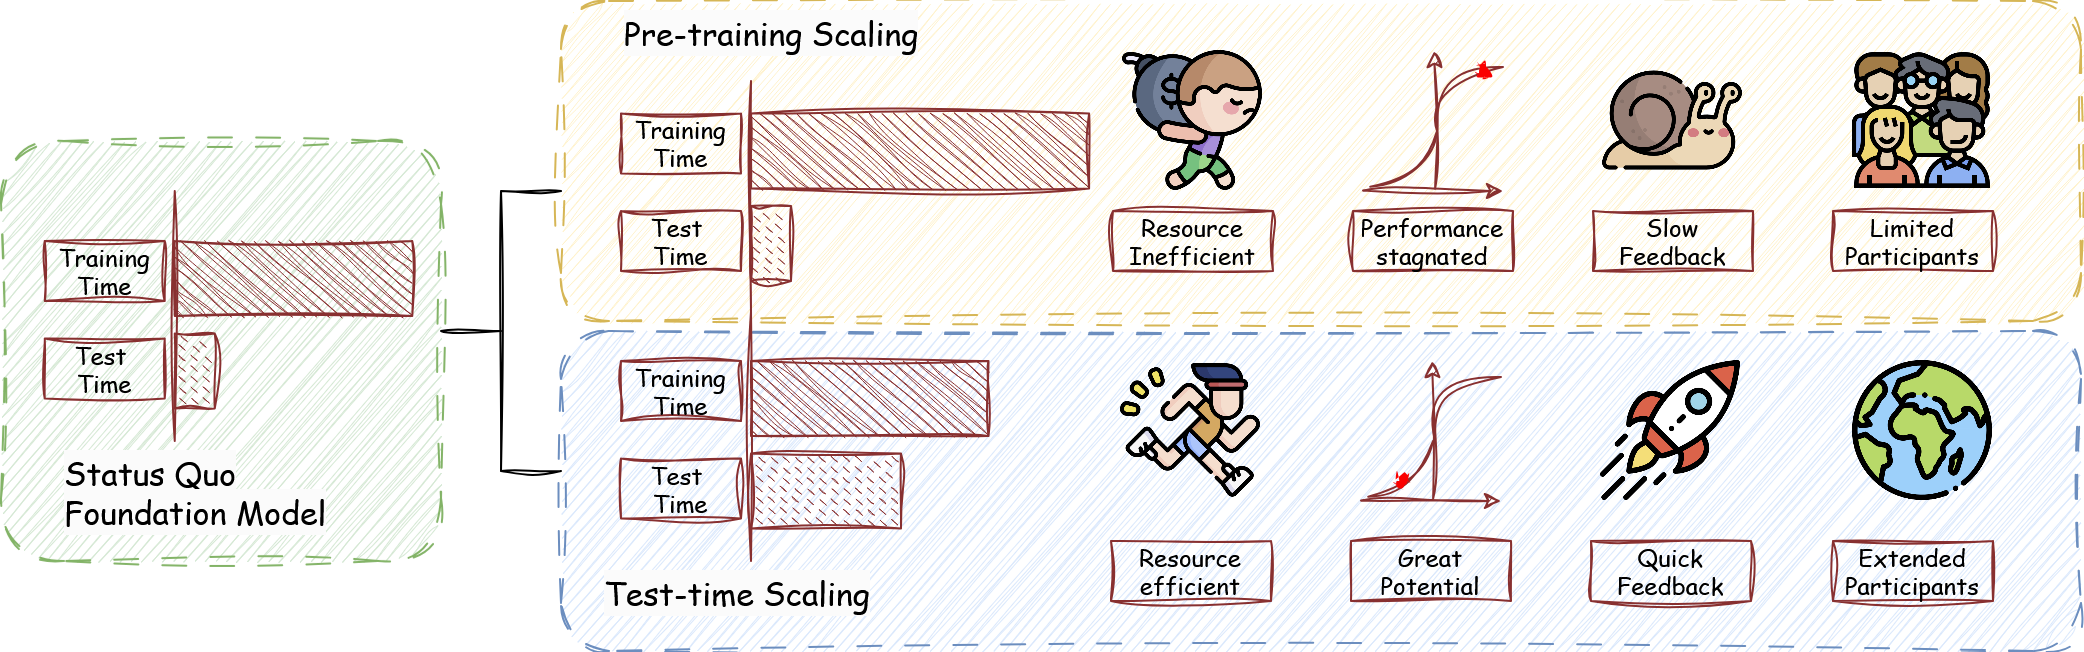
\includegraphics[width=0.98\linewidth]{figures/TTS-intro.png}
    \caption{Comparison of Scaling Paradigms in Pre-training and Test-time Phases.}
    \label{fig:intro}
\end{figure}


Human cognition may suggest a clue. When faced with complex problems, people tend to engage in deeper, more deliberate thinking, often producing better outcomes~\citep{kahneman2011thinking, daniel2003maps, Evans1984-EVAHAA}. 
Inspired by this principle, recent research~\citep{wei2022chain, wang2023selfconsistency} has introduced methods that \emph{allocate additional computation during inference} to boost task performance.
Notably, some studies~\citep{brown2024large, wu2024scaling} observe patterns akin to scaling laws: increasing inference-time compute yields consistent performance improvements.
This family of methods, referred to as \textbf{test-time scaling} (\textbf{\textit{TTS}}), progressively elicits the model’s intelligence in the test-time, as depicted in Figure~\ref{fig:intro}.
The remarkable successes of reasoning models, such as \textit{o1}~\citep{openai-o1} and \textit{R1}~\citep{deepseek-r1},
have further amplified interest in \textit{TTS}, highlighting its potential as a key driver of LLM reasoning and utility.
However, despite this surge in research activity, the field currently lacks a unified and systematic framework to synthesize insights, compare techniques, or identify consistent trends in \TTS. To address this gap, we present a comprehensive survey of \textit{TTS}, offering a hierarchical and extensible framework to analyze methods, map research efforts, and guide future progress.

To the best of our knowledge, this is the first survey to comprehensively examine \textit{TTS} \emph{across multiple orthogonal dimensions}, offering a structured perspective for both theoretical inquiry and practical deployment.
Our framework dissects \textit{TTS} into four key dimensions: \textbf{\textit{what to scale}}, \textbf{\textit{how to scale}}, \textbf{\textit{where to scale}}, and \textbf{\textit{how well to scale}}. Our work emphasizes a fine-grained, decomposition-based understanding of \textit{TTS}. 
While prior efforts have examined \textit{TTS} from specific lenses—such as input modification and output verification~\citep{snell2024scaling}, or through the lens of \textit{System 2 AI} and \textit{Long Chain-of-Thought} (CoT)~\citep{li2025system, ji2025test, chen2025reasoningerasurveylong}—these works are structured around a timeline, tracing the evolution of techniques over time.
We analyze the full pipeline, from scaling formulations and algorithmic mechanisms to task domains and performance dimensions. We provide a structured foundation that allows future research to be seamlessly integrated into our taxonomy, making it easier to understand their contributions. 
Specifically, \textit{what to scale} in Sec.~\ref{sec:what2scale} is about what to be scaled at the inference stage. \textit{How to scale} in Sec.~\ref{sec:how2scale} depicts how they are implemented. We categorize various techniques, recognizing that a single work may involve multiple techniques; 
%For instance, a complex search strategy can be used to generate long CoTs, which are then refined through supervised fine-tuning (SFT) to enhance LLM imitation. 
\textit{Where to scale} in Sec.~\ref{sec:where2scale} covers the tasks and datasets where these techniques are applied. Finally, \textit{how well to scale} inSec.~\ref{sec:howwell2scale} refers to evaluating the different attributions of \textit{TTS} methods. 
%Grounded in our hierarchical taxonomy, we systematically decompose representative works to highlight their contributions and trade-offs in Sec.~\ref{sec:challenges}.
%From this structured analysis, we extract major trends in \textit{TTS} development and offer \emph{hands-on guidance} for real-world deployment. Lastly, we identify persistent challenges and promising research directions for \TTS's future development, including
%advancing test-time scalability, clarifying the fundamental essence of different techniques in \textit{TTS}, broadening generalization to a wider range of downstream tasks, and optimizing \textit{TTS} along more aspects such as efficiency. 
%Our framework dissects \textit{TTS} into four key dimensions: \textbf{\textit{what to scale}}, \textbf{\textit{how to scale}}, \textbf{\textit{where to scale}}, and \textbf{\textit{how well to scale}}.
%It provides a structured foundation that allows future research to be seamlessly integrated into our taxonomy, making it easier to understand their contributions. Specifically, \textit{what to scale} (Sec.~\ref{sec:what2scale}) is what being scaled at the inference stage. \textit{How to scale} (Sec.~\ref{sec:how2scale}) is how they are implemented, We categorize various techniques, recognizing that a single approach may involve multiple techniques. For instance, a complex search strategy can be used to generate long CoTs, which are then refined through supervised fine-tuning (SFT) to enhance LLM imitation. \textit{Where to scale} (Sec.~\ref{sec:where2scale}) covers the tasks and datasets where these techniques are applied. And \textit{how well to scale} (Sec.~\ref{sec:howwell2scale}) refer to evaluating the different attributions of \textit{TTS} methods. 
We further provide fine-grained subcategories under each axis and systematically map representative works to highlight their contributions and trade-offs (Sec.~\ref{sec:organizationandtrends}).
From this structured analysis, we extract major trends in \textit{TTS} development and offer \emph{hands-on guidance} (Sec.~\ref{sec:handon}) for real-world deployment. Grounded in our multi-dimensional taxonomy, we also identify persistent challenges and promising research directions (Sec.~\ref{sec:challenges}): advancing test-time scalability, clarifying the fundamental essence of the effectiveness of different techniques in \textit{TTS}, broadening generalization to a wider range of downstream tasks, and optimizing \textit{TTS} methods along additional dimensions such as efficiency.


\paragraph{Our contributions are threefold:}
\begin{enumerate}
    \item \textbf{A Unified, Multi-Dimensional Taxonomy.} We propose a four-axis taxonomy—\textit{what to scale}, \textit{how to scale}, \textit{where to scale}, and \textit{how well to scale}—that supports structured classification, comparison, and extensibility for \textit{TTS} methods.
    \item \textbf{Systematical Literature Organization and Pragmatic Analysis.} 
    Using our taxonomy, we survey the \textit{TTS} landscape, analyze representative methods, and present guidelines for research application and deployment.
    \item \textbf{Challenges, Insights, and Forward Directions.} Building on our organized perspective, we uncover critical challenges—ranging from advancing scaling to clarifying essence—and outline promising research directions that could shape future progress. Our unified framework facilitates the mapping of these open questions to concrete dimensions of \textit{TTS}, enabling more targeted and impactful advancements.
\end{enumerate}

We plan to continuously update our taxonomy to reflect ongoing progress and provide an evolving foundation for organizing future developments in \textit{TTS} research.